% LaTeX Article Template - customizing header and footer
\documentclass{article}

\newtheorem{thm}{Theorem}

% Set left margin - The default is 1 inch, so the following
% command sets a 1.25-inch left margin.
\setlength{\oddsidemargin}{0.25in}

% Set width of the text - What is left will be the right margin.
% In this case, right margin is 8.5in - 1.25in - 6in = 1.25in.
\setlength{\textwidth}{6in}

% Set top margin - The default is 1 inch, so the following
% command sets a 0.75-inch top margin.
\setlength{\topmargin}{-0.25in}

% Set height of the header
\setlength{\headheight}{0.1in}

% Set vertical distance between the header and the text
\setlength{\headsep}{0.2in}

% Set height of the text
\setlength{\textheight}{9in}

% Set vertical distance between the text and the
% bottom of footer
\setlength{\footskip}{0.1in}

% Set the beginning of a LaTeX document
\usepackage{multirow}
\usepackage{fullpage}
\usepackage{graphicx}
\usepackage{amsthm}
\usepackage{amssymb}
\usepackage{amssymb}
\usepackage{algpseudocode}
\usepackage{caption}
\usepackage{float}
\usepackage{subcaption}
\graphicspath{%
    {converted_graphics/}% inserted by PCTeX
    {/}% inserted by PCTeX
}
%%%%%%%%%%%%%%%%%%%%%%%%%%%%%

\begin{document}\title{Chaos Game Analysis\\ Spring 2017\\ Math-M330}         % Enter your title between curly braces
\author{Steven Myers}        % Enter your name between curly braces
\date{\today}          % Enter your date or \today between curly braces
\maketitle


% Redefine "plain" pagestyle
\makeatother     % `@' is restored as a "non-letter" character

% Set to use the "plain" pagestyle
\pagestyle{plain}

\section*{Introduction to the Chaos Game}

\paragraph{}
The chaos game is an iterative process that will produce an image known as the Sierpenski triangle. The classification of images, like the Sierpenski triangle generated by the chaos game, is a \textit{fractal}. A fractal is an image that is created by a mathematical process. Fractals have unique mathematical qualities that can be reasoned by observation and by generating fractals by hand and by machine. The rules for how to play the chaos game are listed below for reference:
\begin{enumerate}
    \item
    Start by placing three points on a piece of paper. For the best results, try placing the points roughly in the three vertices of an equilateral triangle.
    \item
    Next, select an initial point contained within the area of the vertices, or ontop of the invisibile edges connecting the three verticies you drew.
    \item
    Select one of the three points of the triangle randomly. (You may use a dice or random number generator)
    \item
    Draw a new point halfway between the randomly selected vertice and your initial starting point.
    \item
    Repeat step 3 until a pattern emerges or until satisfied.
\end{enumerate}

\paragraph{}
In the first iterations of the chaos game, it's likely that the generated points fall along defined edges at different angles leading towards the three vertices. This early pattern that one may notice is that the points will follow a "tug-of-war" pattern, moving back and forth between just two the vertices and forming what appears to be a defined edge. You may even begin to notice an upside down triangle circumscribed within our original area between the three vertices. Using a computer program, we can generate more points than what would be possible by pencil and paper. In Figure 1, we can view a few resulting images of the chaos game, generated by a computer program.
\begin{figure}[H]
    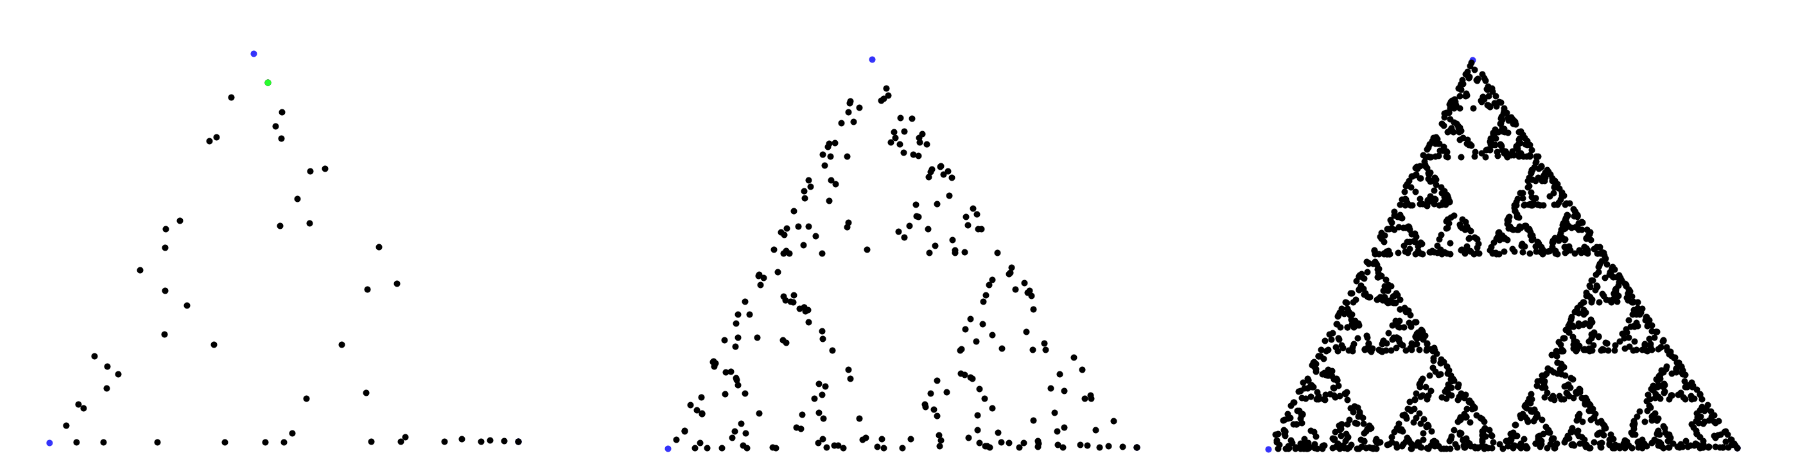
\includegraphics[width=\linewidth, height=.2\textheight]{combined_image}
    \caption{Images created by the Chaos Game for 50, 250, and 1000 iterations respectively.}
\end{figure}
\paragraph{}
Looking at Figure 1, we can immediately see that there are well-defined spaces where no points fall. When we iterate 250 times or more, we begin to see these spaces fully develop as upside down, circumscribed triangles. If we try replay the chaos game by hand and select new initial starting points, we will find that no initial starting point can produce subsequent points within these zones where no points fall, no matter the initial starting point we choose

 So, by iteratively working the chaos game out, we see that a common pattern emerges that is \textit{not} random. We have consistent areas in which no points fall, and we eventually get the same resulting image regardless of our initial starting point.
\section*{The Sierpenski Triangle}
\begin{figure}[H]
    \centering
    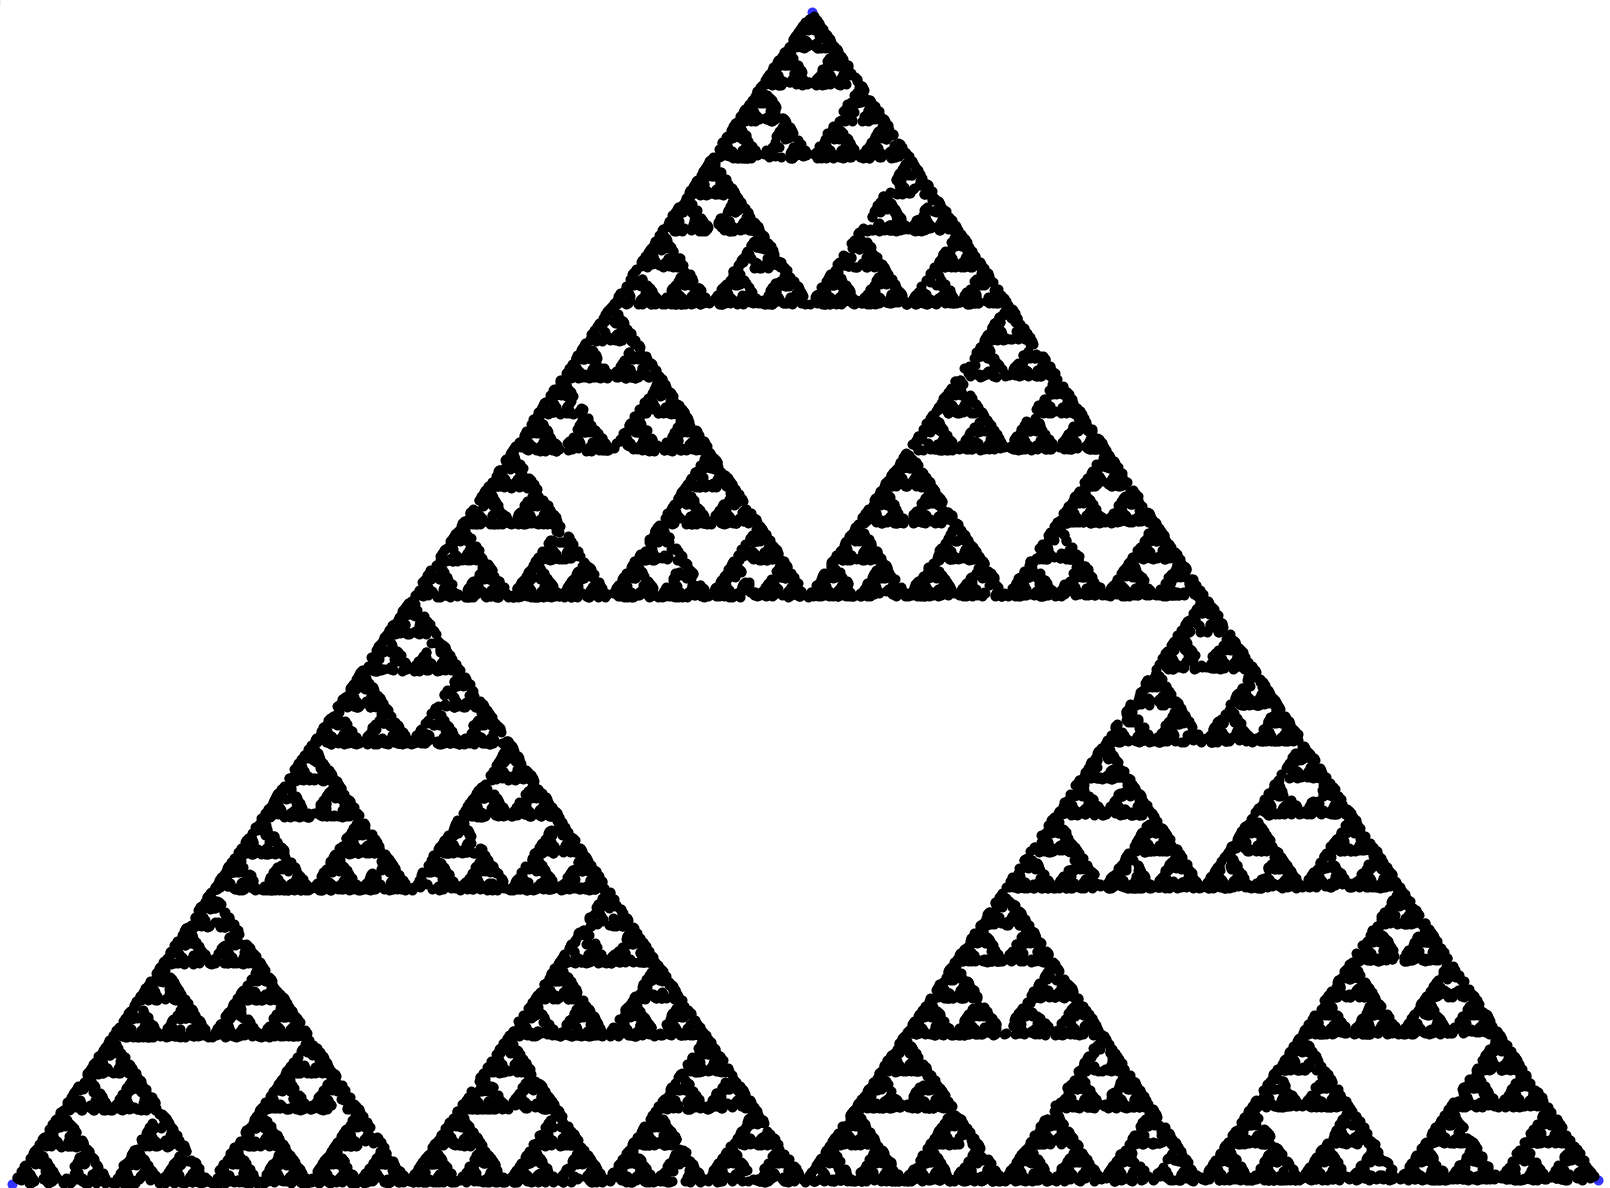
\includegraphics[width=.5\linewidth, height=.25\textheight]{ideal}
    \caption{The ideal Sierpenski triangle shape.}
\end{figure}
\paragraph{}
When the chaos game is iterated infinitely many times, it eventually produces the Sierpenski triangle. In an ideal Sierpenski triangle, all of the edges are fully formed as we can nearly see in the later iterations of the chaos game. Figure 2 shows the fully formed Sierpenski triangle. The Sierpenski triangle has a number of unique qualities that extend beyond how the points fall in the chaos game. It consists of smaller Sierpenski triangles in its three sub-triangles. Subtriangles are formed by the circumscribed upside triangles in the center of each Sierpenski triangle - forming four triangles of 1/4 the surface area of the original triangle. The upside triangle in the center serves as "lost space" where the image is no longer created. We can think of this as lost surface area.
\paragraph{}
Like we did with the chaos game, we can come up with a series of steps to create the ideal Sierpenski triangle shape:
\begin{enumerate}
    \item Draw an equilateral triangle.
    \item Draw an upside down equilateral triangle within the equilateral triangle. This triangle should be 1/4 of the size of the original.
    \item Repeat step 2 indefinitely for the three upright, smaller subtriangles.
\end{enumerate}
\paragraph{}
With this new set of instructions, we can begin to make further observations about the Sierpenski triangle. We can immediately notice that every time we create a new Sierpenski triangle, the original triangle loses a quarter of its surface area. The surface area is \textit{lost} in the sense that no further iterations of the Sierpenski triangle are generated in the upside down triangles. In terms of the chaos game, the surface area is lost since no points will ever fall within the the middle of the triangle. Since the ideal Sierpenski triangle shape continues indefinitely within its subtriangles, and we know that from each iteration a quarter of surface area is lost, we can deduce that the area of the Sierpenski triangles approach a limit of zero surface area. So, we have a shape that essentially has zero surface area.
\end{document}
